\begin{table}[h]
\begin{tabular}{llll}
{Rank} &       Word &        User     &  Mixed \\
\hline
1  &        ushuaia &          chivil &       chivilcoy \\ 
2  &          rioja &            ush  &             ush \\
3  &      chivilcoy &            poec &         tolhuin \\
4  &        bragado &\textbf{malpegue}&             blv \\
5  &         viedma &   \textbf{aijue}&          chivil \\
6  &        logroño &         tolhuin &         logroño \\
7  &         chepes &        vallerga &         bragado \\
8  &          oberá &  \textbf{yarca} &        vallerga \\
9  &  \textbf{cldo} &             blv &          breñas \\
10 &            tdf &          portho &\textbf{malpegue}\\
11 &       riojanos &          jumeal &  \textbf{aijue} \\
12 &         breñas &   \textbf{sinf} &          choele \\
13 &         choele &        plottier &           oberá \\
14 &       gallegos &           kraka &           obera \\
15 &      tiemposur &             fsa &   \textbf{cldo} \\
16 &      fueguinos & \textbf{bombola}&        plottier \\
17 &      chilecito &  \textbf{yarco} &           kraka \\
18 &            blv &       sanagasta &   \textbf{sinf} \\
19 &            ush &            wika &            poec \\
20 &          merlo &           obera &             nqn \\
\hline
% Mixed and User share 12 words
% Mixed and Word share 8 words
\end{tabular}
\caption{Top 20 words for each metric. Words in bold have lexicographic interest as regionalisms.}
% Among these words, \emph{yarca/yarco, aijue, sinf, cldo, bombola, malpegue} have lexicographic interest as they are regionalisms}
\label{tab:20_top_words}
\end{table}

Table \ref{tab:20_top_words} shows the top-20 words calculated with each metric.  Many are toponyms: \emph{chivil, ush, blv, tolhuin, kraka, sanagasta, wika} refer to towns, cities and local clubs. Also, some words refer to gentilics (\emph{riojanos, fueguinos}), or local institutions (\emph{POEC}). Some of these words emerge as regionalisms: \emph{yarca/yarco, aijue, sinf, cldo, bombola, malpegue}. We can observe that many words are shared among the rankings. \userrank*{} and \wordrank*{} have an overlap of 63\%, \userrank*{} and \mixedrank*{} have 83\% words in common, and \userrank*{} and \wordrank*{} share 79\% of their entries.



\begin{figure*}[t!]
   \centering
   \begin{subfigure}[t]{0.49\textwidth}
   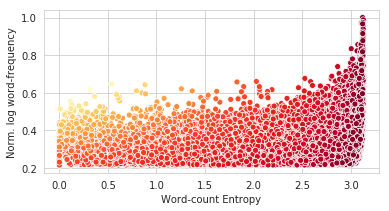
\includegraphics[width=\textwidth]{./images/word_iv_word_axes.png}
   \caption{Color scale: \wordrank{}}
   \label{fig:word_iv_word_axes}
   \end{subfigure}
   \begin{subfigure}[t]{0.49\textwidth}
   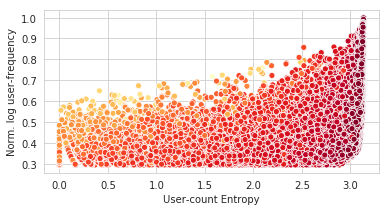
\includegraphics[width=\textwidth]{./images/word_iv_user_axes.png}
   \caption{Color scale: \wordrank{}}
   \label{fig:word_iv_user_axes}
   \end{subfigure}
   % User Information Value
   \begin{subfigure}[t]{0.49\textwidth}
   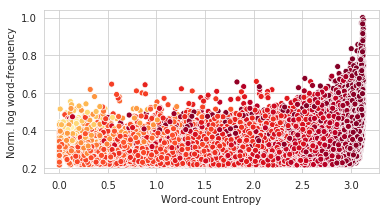
\includegraphics[width=\textwidth]{./images/user_iv_word_axes.png}
   \caption{Color scale: \userrank{}}
   \label{fig:user_iv_word_axes}
   \end{subfigure}
   \begin{subfigure}[t]{0.49\textwidth}
   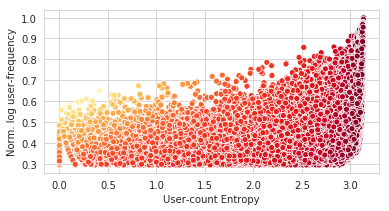
\includegraphics[width=\textwidth]{./images/user_iv_user_axes.png}
   \caption{Color scale: \userrank{}}
   \label{fig:user_iv_user_axes}
   \end{subfigure}
   %Mixed Information Value
%   \begin{subfigure}[t]{0.49\textwidth}
%   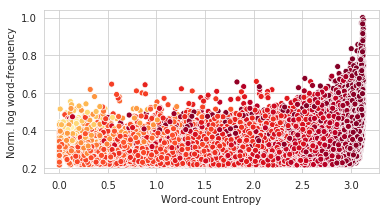
\includegraphics[width=\textwidth]{./images/user_iv_word_axes.png}
%   \caption{Mixed Information Value on Word Axes}
%   \label{fig:mixed_iv_word_axes}
%   \end{subfigure}
%   \begin{subfigure}[t]{0.49\textwidth}
%   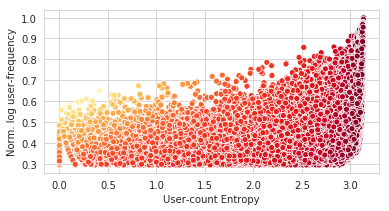
\includegraphics[width=\textwidth]{./images/user_iv_user_axes.png}
%   \caption{Mixed Information Value on Word Axes}

 %  \label{fig:mixed_iv_user_axes}
%   \end{subfigure}
 
   \caption{Scatter plots showing words (dots) along three dimensions. Horizontal axes: word-count entropy $H_\text{words}$ (left plots) or user-count entropy $H_\text{users}$ (right plots). Vertical axes: normalized log word frequencies $n_\text{words}$ (left plots) or user frequencies $n_\text{users}$ (right plots). Color: log word rank according to \wordrank*{} (top plots) or to \userrank*{} (bottom plots); lighter color means higher rank.}
   %Scatter plots of words on entropy and normalized log frequency. Color, the z-axis, represents the logarithm of the rank of the word: lightest points represent most important words, those with top position in the ranking. Left column uses Word-Count Entropy on its x-axis and Normalized log-frequency in y-axis, and right column uses User-Count Entropy and Normalized log-user-frequency. Figures in the first row use \wordrank{} and the second one uses \userrank{}. Figures \ref{fig:word_iv_word_axes} and \ref{fig:user_iv_user_axes} are similar in that they use the same set of axes and rank. Top ranked words tend to be in the top-left corner, that is: low entropy/high concentration, and with a high number of occurrences or users. Figure \ref{fig:word_iv_user_axes} uses user-count axes with \wordrank{} and a slight disorder in the colors can be seen. Figure \ref{fig:user_iv_word_axes}, colored with the logarithm of \userrank{} and in user axes, present more drastic changes in the colours: there are many words that are very low in the Word-Count rank and very high in the User-Count Rank.}
   \label{fig:ivalue}
\end{figure*}



Figure \ref{fig:ivalue} shows four three-dimensional scatter plots. A dot in these plots corresponds to an individual word in our corpus, and is placed along the horizontal axes according to its word- or user-count entropy ($H_\text{words}(\omega)$ and $H_\text{users}(\omega)$, respectively) -- the same horizontal axes shown in Figure \ref{fig:entropies}. Along the vertical axes, each dot is located following its corresponding word or user frequency ($n_\text{words}(\omega)$ and $n_\text{users}(\omega)$). Additionally, each dot is colored according to the position of the word in one of our rankings using a chromatic scale, such that the lighter the dot, the higher the word's rank. For clearer visualization, word rankings are also shown in logarithmic scale.

Figure \ref{fig:word_iv_word_axes} shows that words that figure high in the \wordrank{} (in lighter color) tend to appear closer to the upper-left corner of the plot -- that is, such words are more frequent and their mentions are concentrated in fewer regions. Figure \ref{fig:user_iv_user_axes} shows a very similar thing, now with respect to the number of users that mention the words: words high in the \userrank{} are mentioned by a larger number of users from fewer regions.
These two figures display a gradient from the upper-left corner (words ranked higher, in lighter color) to the lower-right corner (words ranked lower, in darker color). 

Figure \ref{fig:word_iv_user_axes} uses horizontal and vertical axes corresponding to users ($H_\text{users}$ and $n_\text{users}$), but colors each word with respect to \wordrank{}. Here we can observe a slight perturbation in the gradient: there are words far from the left-corner that have light colors. From this, we understand that there are words with high \wordrank{} that have low \userrank{}. 

Likewise, Figure \ref{fig:user_iv_word_axes} uses \userrank{} to color the points, and word axes $H_\text{user}$ and $n_\text{user}$. The perturbation in the gradient is even clearer in this plot: There are many words that appear high in \wordrank{} (closer to the top-left corner, see Figure  \ref{fig:word_iv_word_axes}) but appear low in \userrank{} (darker color). 


To further inspect this phenomenon, we searched for words that have large differences in the logarithm of \wordrank{} and \userrank{}. The logarithm minimizes the difference between words ranked very high (e.g. between the word at position 10,000 and another in position 20,000) and amplifies the difference when one of the ranks is low and the other is high. Table \ref{tab:table_rank_differences} shows the words with the highest differences. We can see that these words rank very high in the word metric, but very low in user rank. A close examination of these words and the tweets they were used in showed that they were in the vocabulary of bots (news and metheorological accounts, or accounts using applications to get more followers) or small niches of fans of a certain celebrity. From the top-100 words sorted by this difference, only one has a higher ranking in users than in words. 

Summing up, when a word has a high \userrank{}, it also tends to have a high \wordrank{}. The reverse is not true, however, as words produced by a small number of accounts would not rank well with respect to users. Thus, the  \userrank{} successfully discards words coming from automatic agents, as already done in \citet{Cui:2012:DBE:2396761.2398519}. This observation also explains the similarities between the \mixedrank{} and \userrank{}, given that the product of the two metrics will be high mainly when \userrank{} is high. We omit the scatterplots for our third metric due to space constraints, because they are very similar to those of the \userrank{}.

\begin{table}[h]
    \centering
        
    \begin{tabular}{lrr}
    Word &  Word Rank &  User Rank \\
    \hline
    rioja         &              2 &           2499 \\
    vto           &             27 &          28179 \\
    hoa           &             81 &          83717 \\
    contextos     &             88 &          71290 \\
    cardi         &             32 &          23756 \\
    agraden       &            107 &          75042 \\
    hemmings      &             59 &          40227 \\
    ushuaia       &              1 &            565 \\
    tweeted       &             43 &          21342 \\
    precipitación &             66 &          31042 \\
    \hline
    \end{tabular}

    \caption{Top 10 words with largest difference between their log word rank and their log user rank.}
     %Most of these words come from automatic bots or applications. For instance, \emph{precipitación, hoa, vto} are words used by bots tweeting metheorological information}
    \label{tab:table_rank_differences}
\end{table}

Table \ref{tab:metric_results} shows the percentage of words marked as being lexicographically interesting. This validation suggests that \userrank*{} is the most relevant ranking when assessing the word as a regionalism. \mixedrank{} occupies the second position due to its high overlap with the first metric.

Lastly, Table \ref{tab:characterisation} displays some groups among the regionalisms found in the analyzed words with examples. A special note is reserved for the group of \emph{Indigenisms}, where a number of words were found coming from \emph{guaraní} (for instance, \emph{mitaí, angá, angaú, nderakore}) and also from \emph{quechua} (\emph{ura}). It is worth mentioning that words coming from \emph{guaraní} —language spoken in Northeastern Argentina, Paraguay, Bolivia and Southwest of Brazil— coincide with the region delimited by \citet{vidal1964espanol}.


\begin{table}[b]
\centering
\begin{tabular}{lr}
Metric                      &  \% of pertinent words  \\ % &           STD \\
\hline
Word-Count       &  21.9\%   \\
User-Count       &  30.2\%  \\
Mixed            &  25.3\%  \\ %&  1.947665e+01 \\
\hline
\end{tabular}
\caption{Results of the metrics. The percentage of detected regionalisms in the first 1000 words is given for each rank: \wordrank{}, \userrank{} and \mixedrank{} }
\label{tab:metric_results}
\end{table}


\newcommand{\tabinterspace}{\newline\newline}

\begin{table}[t]
\centering
Colloquialisms
\begin{tabular}{p{0.1\textwidth} p{0.1\textwidth} p{0.2\textwidth}}
\hline
Word & Region & Meaning \\
\hline
culiado & Córdoba & asshole   \\
chombi & Mendoza &  poor in quality\\
carnasas & Neuquén & not classy, inelegant  \\
bolasear & Cuyo & to bullshit \\
aprontar & E. Ríos& to get ready\\
\hline 
\end{tabular}
\tabinterspace{}
Indigenisms
\begin{tabular}{p{0.1\textwidth} p{0.1\textwidth} p{0.2\textwidth}}

\hline 
ura & Northwest & vagina (quechua)\\
mitaí & Guaranitic & boy \\
angá & Guaranitic & unfortunate \\
\hline 
\end{tabular}
\tabinterspace{}
Regional realities
\begin{tabular}{p{0.1\textwidth} p{0.1\textwidth} p{0.2\textwidth}}
\hline 
piadinas & San Juan & roll (food) \\
tarefero & Misiones & yerba mate worker \\
POEC & Neuquén & high School exam \\ 
\hline 
\end{tabular}
\tabinterspace{}
Interjections
\begin{tabular}{p{0.1\textwidth} p{0.1\textwidth} p{0.2\textwidth}}

\hline
aijue & Formosa & surprise \\
yirr & Corrientes & joy \\
aiss & Formosa & annoy \\
jiaa & Corrientes & yeehay \\
\hline
\end{tabular}
\tabinterspace{}
Ortographic variations
\begin{tabular}{p{0.1\textwidth} p{0.1\textwidth} p{0.2\textwidth}}

\hline 
pesao & Northwest & pesado \\
ql & Northwest & culiado \\
uaso & Córdoba & guaso \\
\hline
\end{tabular}
\tabinterspace{}
Regional Morpheme
\begin{tabular}{p{0.1\textwidth} p{0.1\textwidth} p{0.2\textwidth}}

\hline 
raraso & Córdoba & very strange (raro) \\
tardaso & Córdoba & very late (tarde) \\
\hline 
\end{tabular}
\caption{Characterization of some of the regionalisms found in the analysis. Each group corresponds to a subjective category found by the lexicographers during the annotation process} 

\label{tab:characterisation}
\end{table}
